\documentclass[a4]{article}
\usepackage[utf8]{inputenc}
\usepackage[french]{babel}
\usepackage{listings}
\usepackage{color}
\usepackage{graphicx}
\usepackage[T1]{fontenc}
\usepackage{pdfpages}
\usepackage{geometry}
\geometry{hmargin=2.5cm,vmargin=2.5cm}

\definecolor{mygreen}{rgb}{0,0.6,0}
\definecolor{mygray}{rgb}{0.5,0.5,0.5}
\definecolor{mymauve}{rgb}{0.58,0,0.82}

\lstset{
  backgroundcolor=\color{white},   % choose the background color; you must add \usepackage{color} or \usepackage{xcolor}
  basicstyle=\footnotesize,        % the size of the fonts that are used for the code
  breakatwhitespace=false,         % sets if automatic breaks should only happen at whitespace
  breaklines=true,                 % sets automatic line breaking
  captionpos=b,                    % sets the caption-position to bottom
  commentstyle=\color{mygreen},    % comment style
  deletekeywords={...},            % if you want to delete keywords from the given language
  escapeinside={\%*}{*)},          % if you want to add LaTeX within your code
  extendedchars=true,              % lets you use non-ASCII characters; for 8-bits encodings only, does not work with UTF-8
  frame=L,	                       % adds a frame around the code
  keepspaces=true,                 % keeps spaces in text, useful for keeping indentation of code (possibly needs columns=flexible)
  keywordstyle=\color{blue},       % keyword style
  language=C,                 	   % the language of the code
  otherkeywords={*,...},           % if you want to add more keywords to the set
  numbers=none,                    % where to put the line-numbers; possible values are (none, left, right)
  numbersep=5pt,                   % how far the line-numbers are from the code
  numberstyle=\tiny\color{mygray}, % the style that is used for the line-numbers
  rulecolor=\color{black},         % if not set, the frame-color may be changed on line-breaks within not-black text (e.g. comments (green here))
  showspaces=false,                % show spaces everywhere adding particular underscores; it overrides 'showstringspaces'
  showstringspaces=false,          % underline spaces within strings only
  showtabs=false,                  % show tabs within strings adding particular underscores
  stepnumber=2,                    % the step between two line-numbers. If it's 1, each line will be numbered
  stringstyle=\color{mymauve},     % string literal style
  tabsize=2,	                   % sets default tabsize to 2 spaces
  title=\lstname                   % show the filename of files included with \lstinputlisting; also try caption= instead of title
}
%gestion des caractères latins
\lstset{literate=
  {á}{{\'a}}1 {é}{{\'e}}1 {í}{{\'i}}1 {ó}{{\'o}}1 {ú}{{\'u}}1
  {Á}{{\'A}}1 {É}{{\'E}}1 {Í}{{\'I}}1 {Ó}{{\'O}}1 {Ú}{{\'U}}1
  {à}{{\`a}}1 {è}{{\`e}}1 {ì}{{\`i}}1 {ò}{{\`o}}1 {ù}{{\`u}}1
  {À}{{\`A}}1 {È}{{\'E}}1 {Ì}{{\`I}}1 {Ò}{{\`O}}1 {Ù}{{\`U}}1
  {ä}{{\"a}}1 {ë}{{\"e}}1 {ï}{{\"i}}1 {ö}{{\"o}}1 {ü}{{\"u}}1
  {Ä}{{\"A}}1 {Ë}{{\"E}}1 {Ï}{{\"I}}1 {Ö}{{\"O}}1 {Ü}{{\"U}}1
  {â}{{\^a}}1 {ê}{{\^e}}1 {î}{{\^i}}1 {ô}{{\^o}}1 {û}{{\^u}}1
  {Â}{{\^A}}1 {Ê}{{\^E}}1 {Î}{{\^I}}1 {Ô}{{\^O}}1 {Û}{{\^U}}1
  {œ}{{\oe}}1 {Œ}{{\OE}}1 {æ}{{\ae}}1 {Æ}{{\AE}}1 {ß}{{\ss}}1
  {ű}{{\H{u}}}1 {Ű}{{\H{U}}}1 {ő}{{\H{o}}}1 {Ő}{{\H{O}}}1
  {ç}{{\c c}}1 {Ç}{{\c C}}1 {ø}{{\o}}1 {å}{{\r a}}1 {Å}{{\r A}}1
  {€}{{\EUR}}1 {£}{{\pounds}}1
}
%definition d'un syle pour les documents texte
\lstdefinestyle{txt}{
	frame=none,
	numbers=none,
	stringstyle=\color{black},
}

\begin{document}
	\title{\Huge{\textbf{Cahier Des Charges}}}
	\author{Alabi Steve - Benyamna Younes - Capdenat Nicolas- \\
		Chouipe Thibaut - El Harti Zakaria - Lienhardt Florian \\ \\ \\
		Chef de projet : Benyamna Younes \\ \\ \\ 
		Sous la direction de Mme Kloul \\ \\ \\ \\
		Outil automatique de décryptage \\ \\ \\}
		

	\begin{titlepage}
		\maketitle
		\vspace{20em}
		\begin{center}
\includegraphics{logo_uvsq.jpg}\end{center}
	\end{titlepage}
	\section{Preambule}
			La steganographie, qui est "l'ancêtre" de la cryptographie. Elle se définit comme l'art de cacher un message dans un autre message. Cet "art"
			est appelé art de la dissimulation. 
			Par exemple ,la lettre de Georges Sand à Alfred Musset( la subtilité réside ici dans le fait qu'il faut lire une ligne sur deux de la lettre pour découvrir le vrai message).
			Cependant, cet art présente une importante contre-mesure. En effet, si le message dissimulé est decouvert, le contenu secret esr revelé.

			Ainsi, un autre "art" s'impose: il est appelé art du secret et c'est justement la cryptographie.
			signifiant lui "écrire". En effet, comme le dit Ronald Rivest, grand cryptologue américain et l'un des 3 inventeurs de l'algo
			de crypto à clé publique RSA, la crypto est la pratique et études des techniques pour assurer des communications sûres en présence d'adversaires.
			Trois critères doivent etre respectés : 
			-confidentialité : personne ne doit lire le message et on doit protéger le contenu.
			-authenticité : personne ne doit contrefaire l'origine du message et on doit s'assurer de la 							provenance de celui-ci.
			-intégrité : personne ne doit modifier le message et on doit s'assurer de la non-modification 							de celui-ci.

			La cryptographie, ainsi que la cryptanalyse(tout simplement l'art de rendre clair un texte crypté sans avoir connaissance de la clef utilisée) constituent la cryptologie.
			C'est un art ancien qui a commencé au 16eme siècle avant J-C et c'est egalement une science nouvelle car elle est encore utilisée de nos jours dans plusieurs domaines tels que les banques(cartes), le web(navigateurs)..etc\\
			Au 21éme siecle, une nouvelle forme de cryptographie liée a l'ère de l'informatique est apparue.
			
			Voici ci-dessous un tableau récapitulatif des différents chiffrements les plus connus :
			\\
			\begin{center}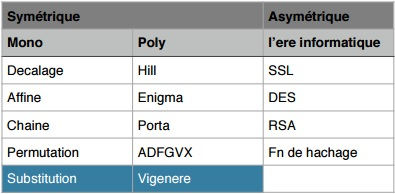
\includegraphics[scale=0.6]{Tab1.jpg}\end{center}
	
	\section{Explications du chiffre de Vigenère et du chiffrement par substitution}
		Nous allons lors de nôtre projet nous interesser aux deux chiffrements suivants.\\
		Pré-condition : Avoir un texte suffisament grand. 
		\subsection{Analyse Fréquentielle}
			L'analyse frequentielle compte le nombre de lettres du texte pour détérminer
			sa taille et compte le nombres d'occurences de chaques lettres.
			Elle calcule ensuite la probabilité d'apparition de chaque lettre.
			Enfin elle compte le nombre des digrammes et trigrammes les plus utilisés.
		\subsection{Vigenère}			    
			\subsubsection{Chiffrement}
				Soit pour chaque lettre de l'alphabet son indice lui correspondant(a=0,b=1..z=25).\\
				Le chiffrement de Vigenère consiste à additionner les valeurs de chaque lettre du texte
				clair avec celles d'un mot-clé qui va se repeter.\\
				Au résultat on appliquera un modulo 26 afin d'être sûre de retomber sur une valeur 
				numérique(entre 0 et 25),
				 et donc correspondant a une lettre de l'alphabet.

			\subsubsection{Dechiffrement}
				Le dechiffrement de Vigenère est basé sur une méthode d'attaque statistique.\\
				On commence par effectuer le test de Kasiski : on cherche des paires de chaines de 
				caractères identiques de longueur > 2 dans le texte chiffré et 
				on note la distance entre les premiers caractères D1.\\
				 Si l'on obtient plusieurs distances D1, D2, .. Di, alors on peut conjecturer que le
				  PGCD des Di est la taille m de la clef.\\
				Ensuite, on va chercher les caractères qui composent notre mot-clef. Nous allons 
				utiliser l'indice de coincidence. Dans une langue usuelle, 
				les lettres n'apparaissent pas toutes avec la même fréquence. C'est pourquoi l'indice 
				de coincidence d'un texte en francais 
				(=If) est très supérieur à l'indice de coïncidence d'un texte aléatoire (=Ia) où les 
				lettres ont une fréquence d'apparition identiques.
				 Ainsi une analyse statistique sur de nombreux textes a donné If=0,074, tandis qu'un 
				 petit calcul donne Ia=0,038 (=1/26)
				Pour chaque caractère du mot clé, on va faire le Mg correspondant à une lettre sur 
				m sur le texte a décrypter. ( 0 < g <25)\\ \\
				$M_{g} = \sum_{i=0}^{25} \frac{P_{i} F_{i+g}}{n^{'}}$\\
				n' = n/m\\
				Pi = probabilité d'apparition d'une lettre dans un texte en francais\\
				Fi = Frequence d'apparition d'une lettre dans un texte chiffré\\ \\
				On va donc obtenir un tableau de m lignes contenant chacunes 26 valeurs et remarquer 
				que une seule valeur par colonne se
				rapproche de 0,074(=If).\\
				On va donc pouvoir en deduire les valeurs des caractères du mot-clé.
				Pour finir, on va soustraire le mot-clef (on le repete autant de fois que nécessaire)
				 au texte chiffré afin d'obtenir le texte clair.
		\subsection{Substitution}
		
			\subsubsection{Chiffrement}
				La méthode de cryptage par substitution  monoalphabétique consiste a remplacer dans un 
				message en clair chaque lettre 
				de l’alphabet de ce message par une lettre d’un alphabet donné. Deux lettres distinctes 
				de l’alphabet du message en clair 
				doivent être chiffrés par deux lettres distinctes de l’alphabet donné afin d’éviter
				 toute ambiguïté lors du déchiffrement.

			\subsubsection{Dechiffrement}
				Le  décryptage de la substitution monoalphabétique est basé sur une  méthode d’attaque
				 statistique utilisant l’analyse fréquentielle.
				Il faut donc que le texte crypté soit assez long pour une analyse statistique.
				On compare ensuite les résultats de l’analyse fréquentielle aux nombres d’occurrences
				de chaque lettre de l’alphabet en clair. Il faut donc connaître la langue correspondant 
				au texte a décrypter. 
				On conjecture alors les correspondances entre les lettres de l’alphabet en clair et de 
				l’alphabet crypté.
				On complète ensuite cette correspondance grace a une analyse des digrammes et des
				trigrammes les plus utilisés dans la langue de
				l’alphabet en clair.
				On possède alors un message partiellement décrypté du message en clair.
				
	\section{Numerotation des exigences}
		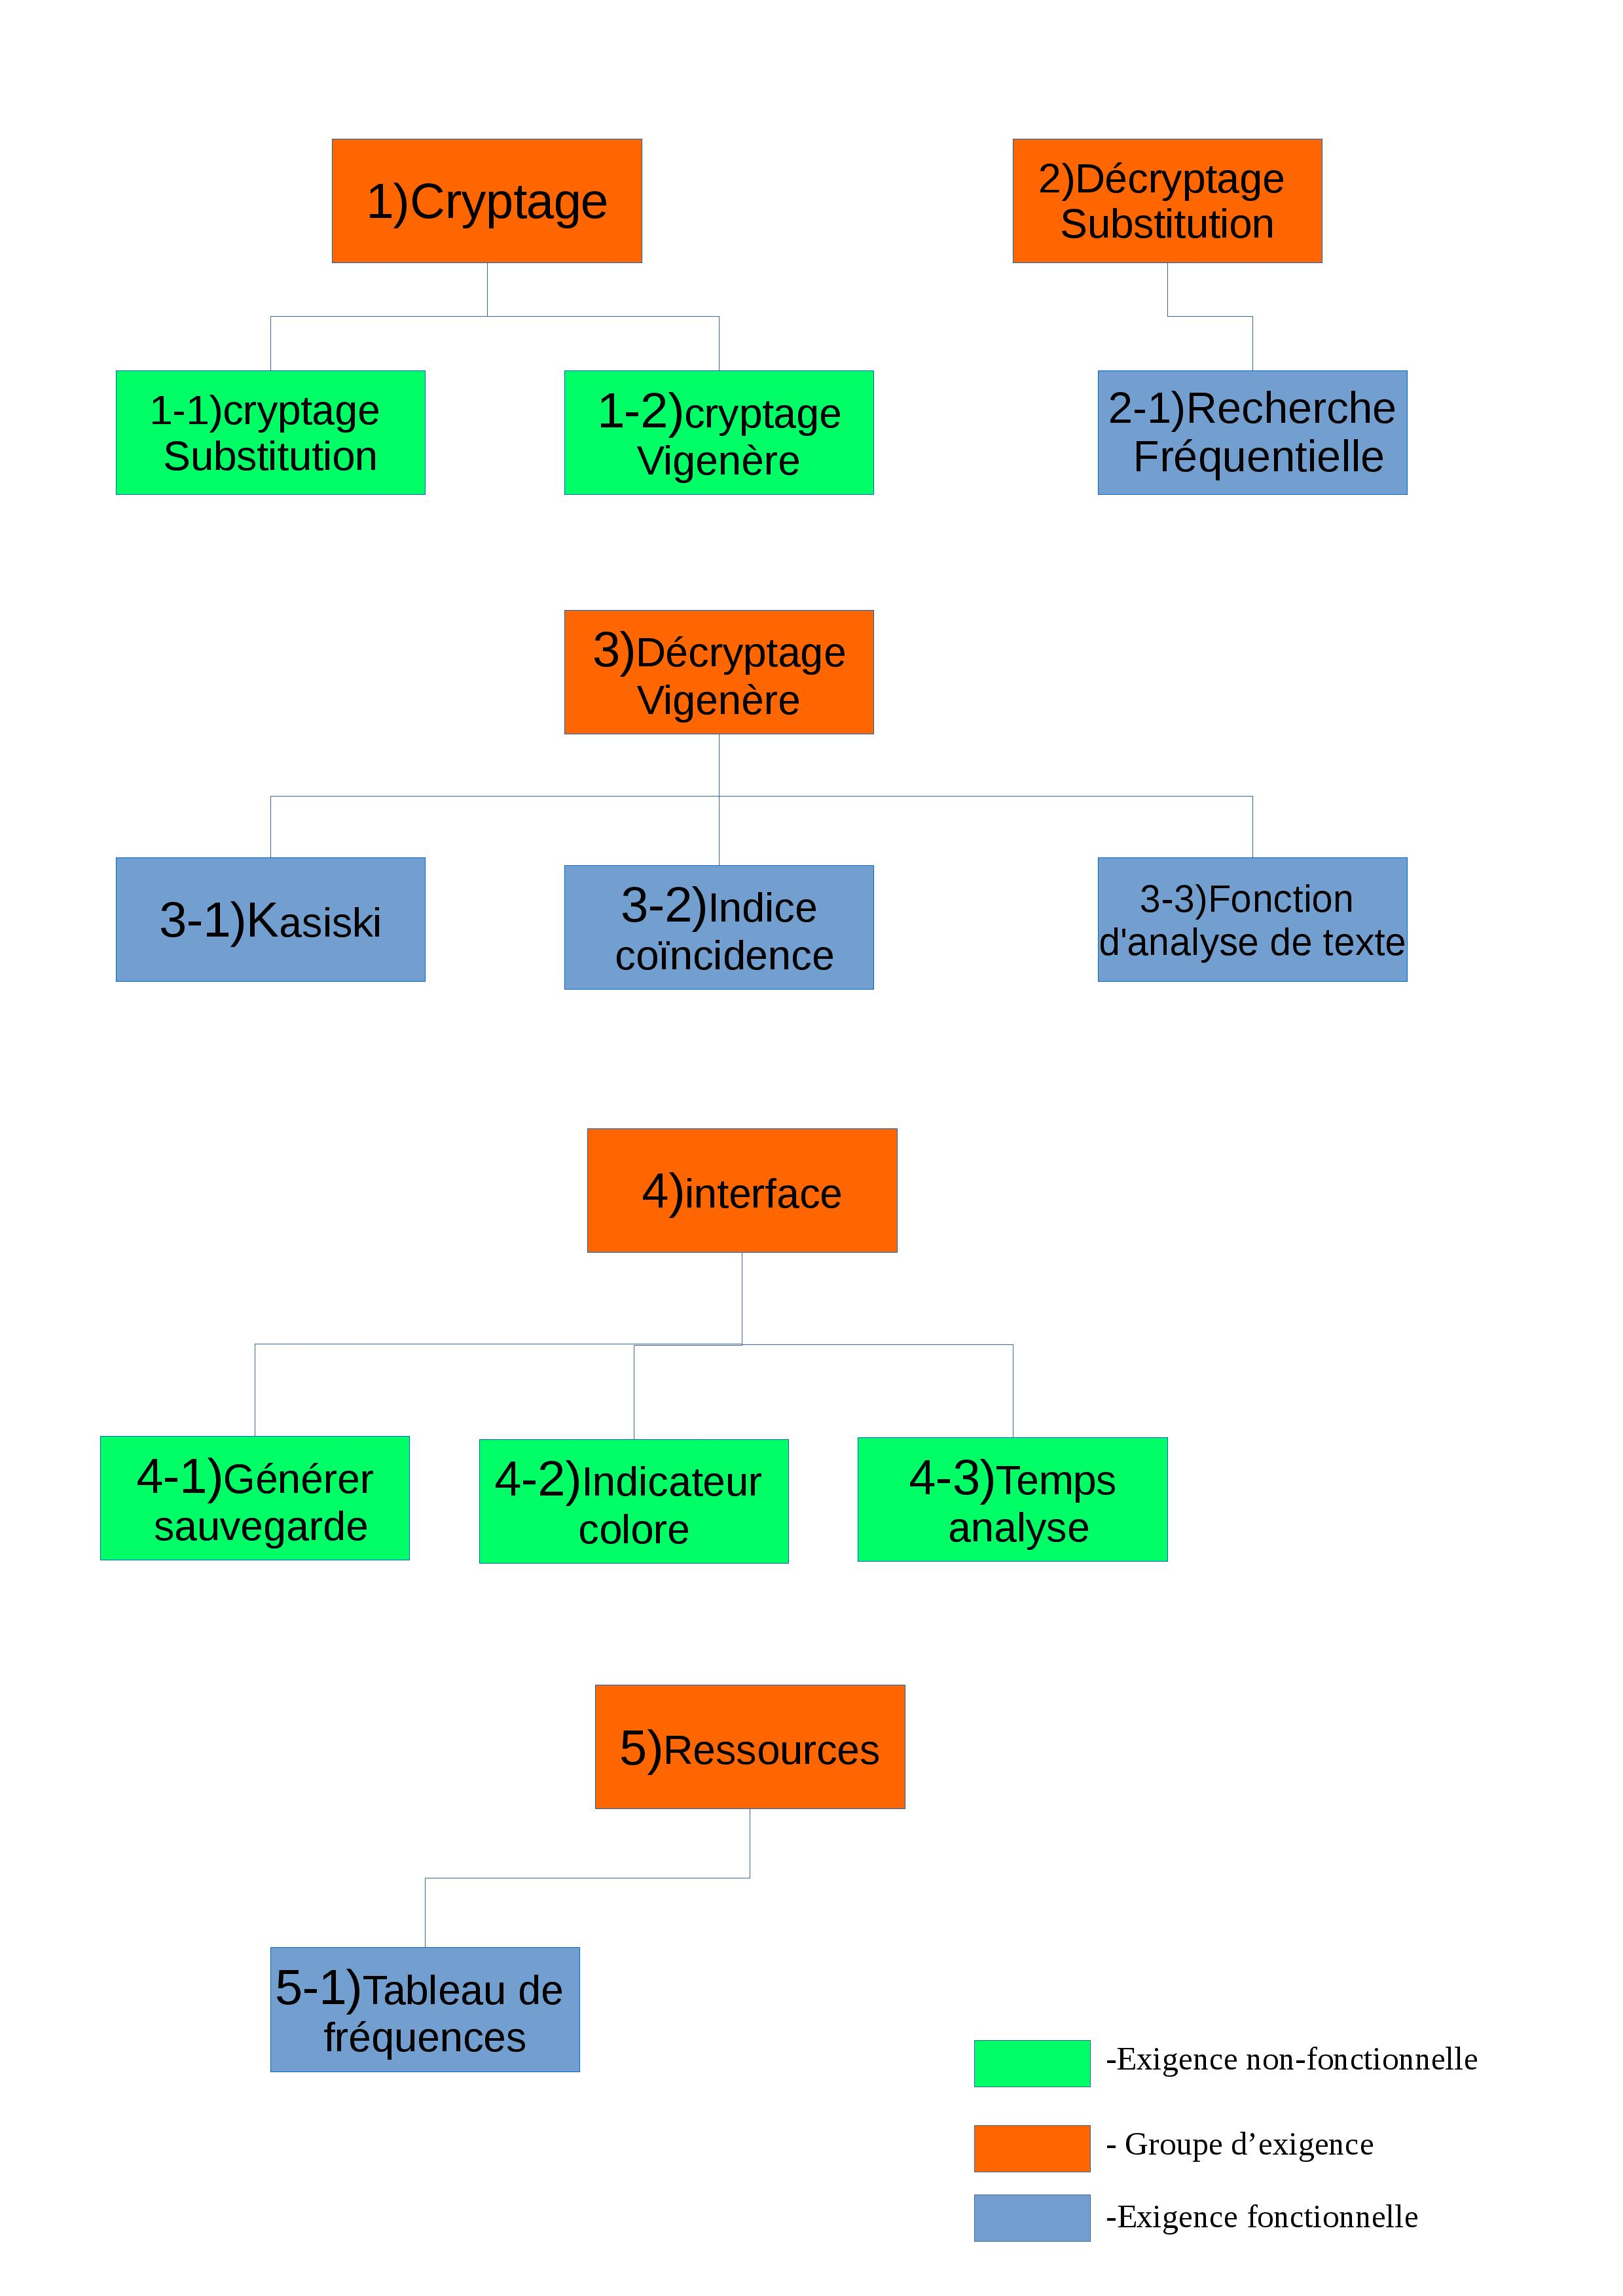
\includegraphics[scale=0.25]{Arbr.jpg} 
		
	\section{Fondement du projet}
		\subsection{Problème de l'utilisation ou contexte du projet}
			Dans le cadre de notre L3, nous devons concevoir un programme d'aide au decryptage.
			Grace a notre programme le client(ici notre enseignante Mme Kloul) va évaluer nôtre travail.
		\subsection{Objectif de la section}
			L'objectif de ce module est de nous apprendre a travailler efficacement en equipe afin 
			de fournir un travail commun.
		\subsection{Objectif du projet}
			Le but du projet est de réaliser un logiciel automatique d'aide au décryptage, capable
			de retrouver une grande partie du texte d'origine à partir d'un texte chiffré. Il devra
			aussi être capable de déchiffrer le chiffrement de Vigenère et le chiffrement par 
			substitution.
	\section{Contraintes sur le projet}
		\subsection{Contraintes sur la conception de la solution}
			-Le produit doit permettre à l'utilisateur de décrypter une partie d'un message crypté.
			-Le produit doit crypter ou décrypter un chiffrement de Vigenère et un chiffrement par 
			substitution.
			-Toutes les deadlines concernant l'application et son cahier des charges doivent être
			 respectées.
		\subsection{ De combien de temps les développeurs disposent-ils pour le projet ?}
			La deadline pour les développeurs est le Vendredi 12 Juin 2017.
		\subsection{Conventions de dénomination}
			k est la clé
			m est la taille de la clé
			n est la taille du message chiffré

	\section{EXIGENCES FONCTIONNELLES}
		\subsection{Portée du produit : cas d’utilisation}
			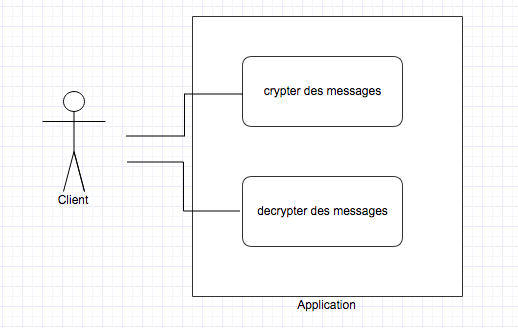
\includegraphics[scale=0.35]{dia.png} \\
			Dans cette application il n'y a qu'un seul type d'utilisateur qui est le client 
			et qui peut crypter et decrypter avec deux méthodes différentes à disposition.
			Il pourra également faire une analyse fréquentielle sur le texte donné.
	\section{EXIGENCES NON FONCTIONNELLES}
		\subsection{Ergonomie et convivialité du produit}
				L'interface permettra de rentrer facilement le texte à décrypter, par copier-coller 
				par exemple.
				De plus, l'interface permettra de choisir la langue (anglais, français) grâce à un
				simple menu.
				Enfin, l'interface permettra aussi d'afficher facilement le resultat obtenu.
				Le programme sera évalué par la responsable du module Projet de la L3 donc il doit 
				apparaître simple et effiace (pas de superflu).
				Le programme ne doit pas être trop gros en terme de resolution, on doit pouvoir 
				l'afficher sur 	tous les types d'écrans d'ordinateurs.
		\subsection{Facilité d’utilisation}
				Le programme sera simple à utiliser même pour un enfant.
				Le programme pourra etre utilisé par des personnes sans qu'elles y soient formées.
		
	\section{AUTRES ASPECTS DU PROJET}
		\subsection{COTS : progiciels et composants commerciaux}
			Il existe sur le marché pas mal de produits pouvant être des solutions potentielles/de remplacement:
			-www.dcode.fr: site proposant de decrypter votre texte. \\
			-Decrypto: disponible sur le Google Play Store et gratuit.\\
			-Axcrypt: logiciel gratuit.
		\subsection{Tâches à faire pour livrer le système}
			Phase I: Identification du projet : La demande du client est clarifiée, les objectifs
			 précisés et dans sa globalité le projet est identifié.\\
			Phase II: Definition du projet : Son contenu est defini de maniere tres precise et la
			 planification des echeances et de la repartition du travail est etablie.\\
			Phase III: Realisation : On realise le projet en adequation avec les exigences du 
			clients et selon le plan de travail defini au prealable.\\
			Phase IV: Finalisation : Le produit est evalué puis remis au client.
			
			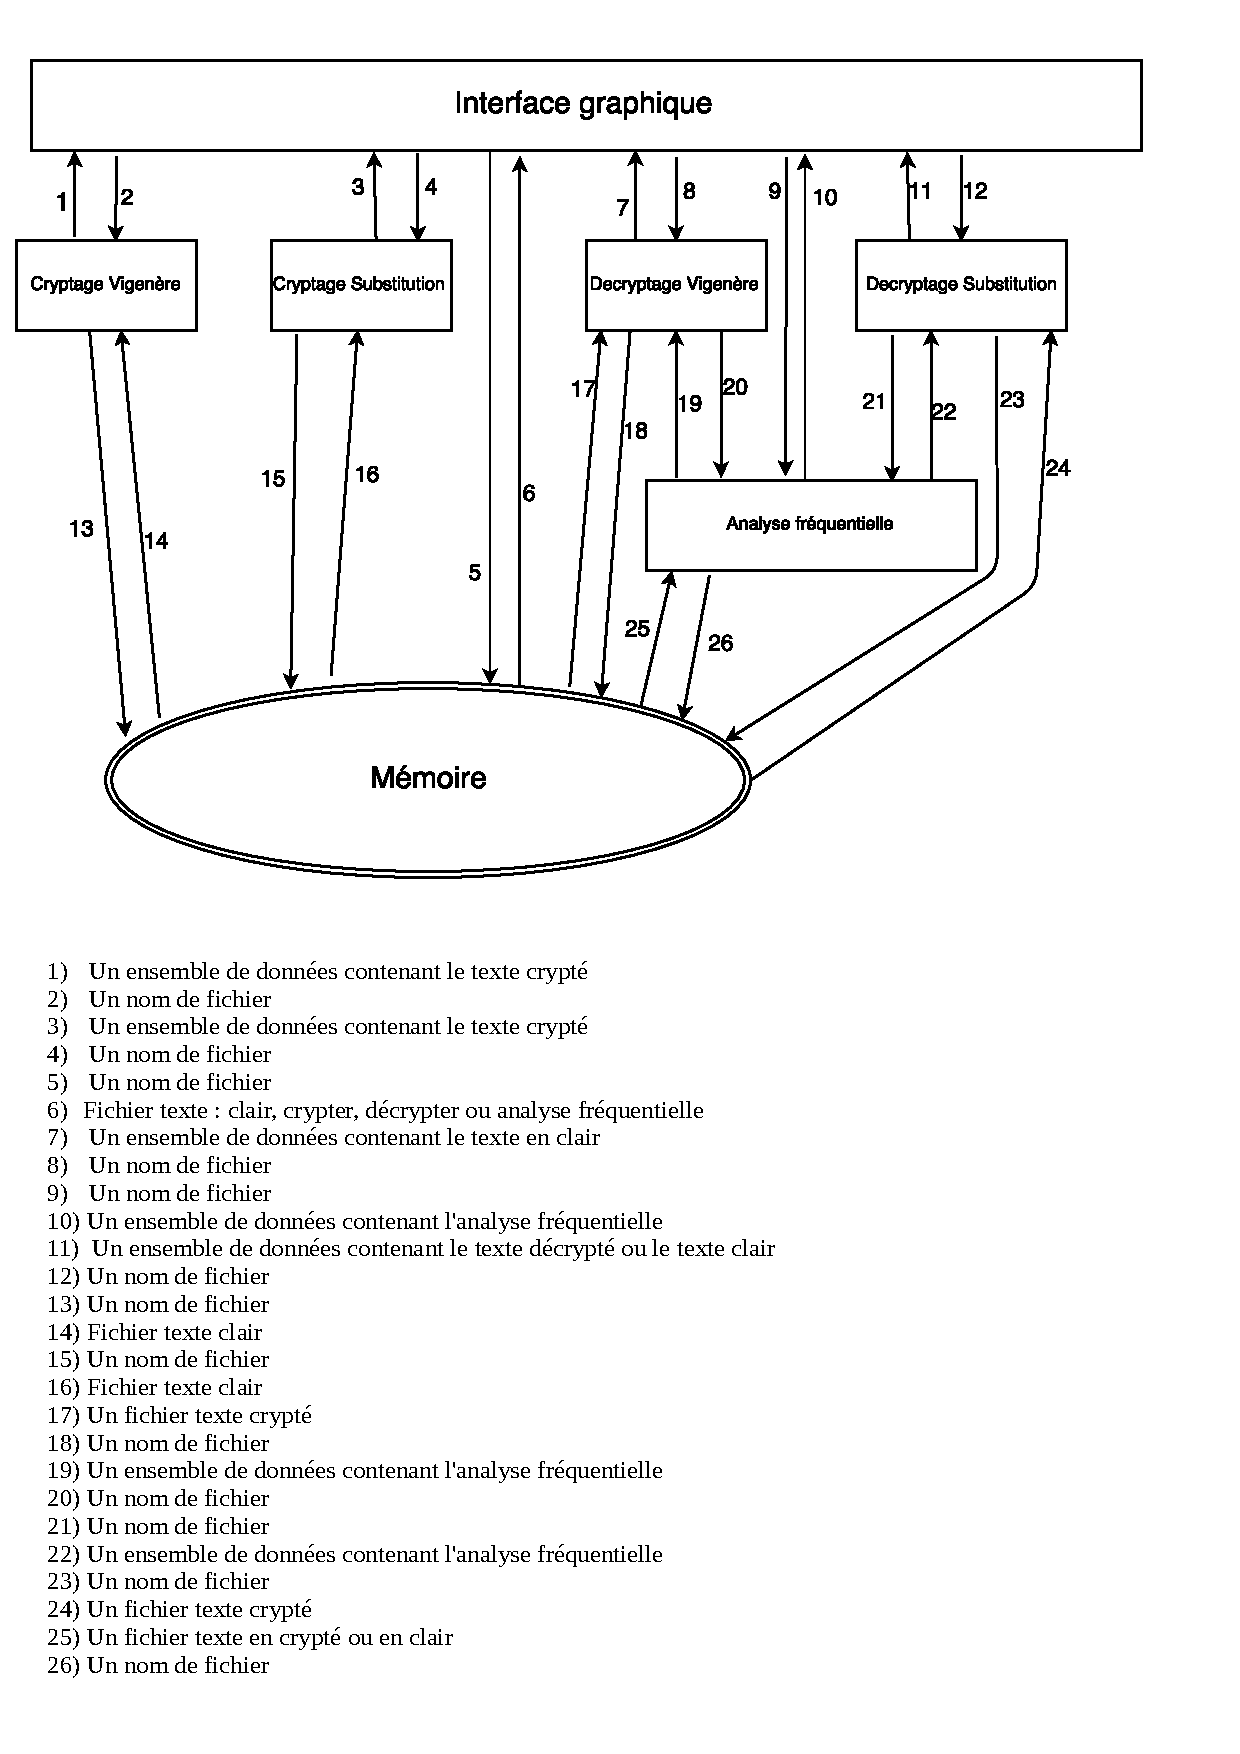
\includepdf[scale=0.7]{organigramme_final.pdf}
			
		\subsection{Organigramme}
			\underline{Interface graphique :}     \hspace{5cm}  \underline{Cryptage Substitution :}\\
			- bouton cryptage            \hspace{5.5cm}       -créer une clé aleatoirement\\
			- bouton decryptage         \hspace{5cm}        -crypter le message\\
			- bouton substitution\\
			- bouton Vigenère           \hspace{5.2cm}       \underline{Cryptage Vigenère :}\\
			- affichage de texte(complet et partiel)  \hspace{2.2cm} -crypter le message\\
			- affichage pour la clé de substitution\\
			- bouton Francais(decryptage)   \hspace{3.5cm}     \underline{Decryptage Substitution :}\\
			- bouton Anglais(decryptage)    \hspace{3.5cm}     -decrypter le message\\
			- affichage pour l'analyse fréquentielle\\
			- charger un fichier texte       \hspace{4.2cm}  \underline{Analyse fréquentielle :}\\
			- sauvegarder un fichier texte     \hspace{3.8cm}  -analyse frequentielle sur texte donné\\
			- créer un nouveau fichier texte(resultats)\\
			- Demander clef de Vigenère\\
			\underline{Decryptage Vigenère :}\\
			-decrypter le message
			
		\subsection{Estimation des coûts du projet}
			\begin{center}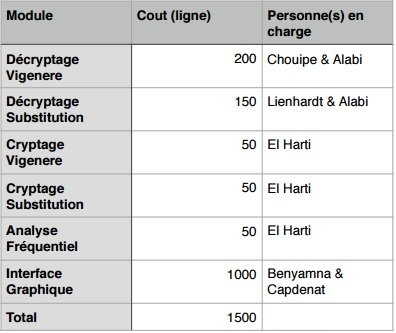
\includegraphics[scale=0.5]{Tableau_cout.jpg}\end{center} 
		\subsection{Manuel utilisateur et formations à envisager}
			L'utilisateur aura accés à un menu lui permettant de choisir de crypter ou décrypter un 
			texte,
			puis la méthode qu'il veut utiliser pour ce faire (vigenere ou substitution), il ne lui 
			restera 
			plus qu'a importer son texte.
		\subsection{Salle d’attente : idées pour les futures versions}
			Bien que le programme ait été demandé que pour la langue francaise et anglaise, 
			il sera sans doute possible d'ajouter d'autres langues dans des versions futurs. 
			Il pourra être également possible d'ajouter une option permettant à l'utilisateur
			d'entrer un type de texte (poème, roman, ordre militaire,...) pouvant aider au décryptage.
			 Ou même encore conserver un historique des "dechiffrements" ou aussi permettre a 
			 l'application de savoir directement si l'on va crypter ou decrypter un texte.
		
	\section{Choix du language}
		Après l'analyse des besoins et après avoir constaté que la programmation 
		orienté-objet n'etait pas nécessaire, nous avons donc choisi d'utiliser le langage C.
		C'est en effet un langage procédurale et performant.
		De plus, toute l'equipe le maitrise, entrainant ainsi une diminution des coûts liée a
		un eventuel temps de formation.
		La bibliothèque graphique que nous avons décidée d'utiliser avec ce langage est GTK+ 
		parce qu'elle permet d'implémenter des boutons, des zones de texte et du traitement de fichier.
		Elle nous semblait donc la plus adaptée au developement de notre application.
	
	\section{Conclusion}
		Afin de répondre aux attentes/besoins du client, nous proposons l'application Dcrypt.
		Elle permet de décrypter facilement un texte chiffré avec le chiffrement de Vigenère ou de 
		Substitution. Cette application permettra également au client de réaliser une analyse fréquentielle sur 
		un texte chiffré. D'autre part elle permettra de chiffrer un texte clair avec le chiffrement de Vigenère ou de
		Substitution. \\
		Ce cahier des charges a été réalisé par une équipe de 6 étudiants de licence en informatique.
		Etant le premier cahier des charges pour chacun de nous, cela nous a permis de nous
		projeter dans une situation plus professionnelle et d'avoir une organisation de travail
		différente suivant un modèle bien précis (ici, Volère).
		
	\newpage
	\section{Sources}
		\textit{Liens(Sites):}\\
		fr.wikipedia.org/wiki/cryptographie\\
		fr.wikipedia.org/wiki/cryptanalyse\\
		fr.wikipedia.org/cryptologie\\
		e-campus.uvsq.fr/cours/chribour/cours-chribour-20140220133009\\
		www.thawte.fr/assets/documents/guides/history-cryptography.pdf\\
		mantis.free.fr/articles/analyse.htm\\
		https://fr.slideshare.net/mobile/antoningaunaud/les-4-phases-du-management-de-projet-2889991\\
		www.volere.co.uk/template-fr\\
		www.bibmath.net/crypto

		\textit{Livres :}\\
		Cryptographie: Théorie et pratique, de Douglas Stinson\\
		Cryptologie et codage: comprendre les codes secrets, de Pierre Vigoureux

\end{document}
